\documentclass[12pt, a4paper]{article}
\title{Homework 4: ICP Fusion}
\author{Christopher Klammer \\ \small\texttt{cklammer@andrew.cmu.edu}}

% A pretty common set of packages
\usepackage[margin=2.5cm]{geometry}
\usepackage[T1]{fontenc}
\usepackage{graphicx}
\usepackage{amssymb}
\usepackage{amsmath}
\usepackage{bm}
\usepackage{color}
\usepackage{float}
\usepackage{bm}
\usepackage{physics}
\usepackage{subcaption}

\begin{document}
\maketitle

\section{Iterative Closest Point}
\subsection{Projective Data Association}
\subsubsection{Conditions for First Filter}
When projecting the source points onto the target points:
\begin{itemize}
    \item The projected source points must lie on the target image plane:
    
    \begin{itemize}
        \item $u \geq 0$
        \item $v \geq 0$
        \item $u \le H$
        \item $v \le W$
    \end{itemize}

    \item The projected source points must be in front of the camera:
    \begin{itemize}
        \item $d(u,v) > 0$
    \end{itemize}
\end{itemize}
\subsubsection{Second Filter Discussion}
The second filter will see if the corresponding 3D points are close enough. Essentially, this is to see if the correspondence is valid. This is necessary because when there are large angles between frames and potential parallax, this check essentially makes sure that the small angle assumption is witheld. Otherwise, We could get two points that have very different depth values and would likely not yield a good solution because it is outside the assumption.
\subsection{Linearization}

\subsubsection{Expansion}
$$p'_i = R^0p_i + t^0$$

$$r_i(\delta R,\delta t) = n^T_{q_i} (\delta Rp'_i + \delta t - q_i)$$

$$
r_i(\delta R,\delta t) = \vert\vert n^T_{q_i} 
(
\begin{bmatrix}
1 & -\gamma & \beta \\
\gamma & 1 & -\alpha \\
-\beta & \alpha & 1    
\end{bmatrix}
\begin{bmatrix}
    (p')_i^x \\
    (p')_i^y  \\
   ( p')_i^z
\end{bmatrix}
+
\begin{bmatrix}
    t_x \\
    t_y \\
    t_z
\end{bmatrix}
-
\begin{bmatrix}
    q_i^x \\
    q_i^y \\
    q_i^z
\end{bmatrix}
)
$$

$$r_i(\delta R,\delta t) = n^T_{q_i} 
(
\begin{bmatrix}
    (p')_i^x - \gamma (p')_i^y  + \beta( p')_i^z + t_x - q_i^x \\
    (p')_i^x \gamma + (p')_i^y  -\alpha( p')_i^z + t_y - q_i^y \\
    -\beta (p')_i^x + \alpha (p')_i^y  +( p')_i^z + t_z - q_i^z
\end{bmatrix}
)
$$


$$r_i(\delta R,\delta t) = n^T_{q_i} 
(
\begin{bmatrix}
    (p')_i^x - \gamma (p')_i^y  + \beta( p')_i^z + t_x - q_i^x \\
    (p')_i^x \gamma + (p')_i^y  -\alpha( p')_i^z + t_y - q_i^y \\
    -\beta (p')_i^x + \alpha (p')_i^y  +( p')_i^z + t_z - q_i^z
\end{bmatrix}
)
$$

$$
r_i(\delta R,\delta t) =
    n^x_{q_i} * ((p')_i^x - \gamma (p')_i^y  + \beta( p')_i^z + t_x - q_i^x)  +
    n^y_{q_i} * ((p')_i^x \gamma + (p')_i^y  -\alpha( p')_i^z + t_y - q_i^y)  +
    n^z_{q_i} * (-\beta (p')_i^x + \alpha (p')_i^y  +( p')_i^z + t_z - q_i^z)
$$

\subsubsection{Formulate into $r_i = Ax + b$}
\paragraph{Variables in A:}

$$n^x_{q_i} (-\gamma (p')_i^y  + \beta( p')_i^z + t_x)$$

$$n^y_{q_i}((p')_i^x \gamma -\alpha( p')_i^z + t_y)$$

$$n^z_{q_i} (-\beta (p')_i^x + \alpha (p')_i^y  + t_z)$$

$$
A = 
\begin{bmatrix}
    -n^y_{q_i}( p')_i^z + n^z_{q_i} (p')_i^y  \\
    n^x_{q_i}( p')_i^z - n^z_{q_i} (p')_i^x \\
    -n^x_{q_i} (p')_i^y  + n^y_{q_i} (p')_i^x  \\ 
    n^x_{q_i} \\
    n^y_{q_i} \\
    n^z_{q_i}
\end{bmatrix}^T
$$
\paragraph{Variables in b:}

$$b_1 = n^x_{q_i} ((p')_i^x -q_i^x)$$
$$b_2 = n^y_{q_i} ((p')_i^y  - q_i^y)$$
$$b_3 = n^z_{q_i} ((p')_i^z - q_i^z)$$

\paragraph{Final Form:}
$$r_i = \begin{bmatrix}
    -n^y_{q_i}( p')_i^z + n^z_{q_i} (p')_i^y  &
    n^x_{q_i}( p')_i^z - n^z_{q_i} (p')_i^x &
    -n^x_{q_i} (p')_i^y  + n^y_{q_i} (p')_i^x &
    n^x_{q_i} &
    n^y_{q_i} &
    n^z_{q_i}
\end{bmatrix}
\begin{bmatrix}
    \alpha \\
    \beta \\
    \gamma \\
    t_x \\
    t_y \\
    t_z
\end{bmatrix}
+
(b_1 + b_2 + b_3)
$$

As the pdf alludes to, we can use the cross-product matrix to simplify the derivation

$$[p']_{\cross} = 
\begin{bmatrix}
    0 & -(p')_i^z & (p')_i^y \\
    (p')_i^z & 0 & -(p')_i^x\\
    -(p')_i^y  & (p')_i^x & 0
\end{bmatrix}
$$

$$
C =
[p']_{\cross}
\begin{bmatrix}
    n^x_{q_i} \\
    n^y_{q_i} \\
    n^z_{q_i} 
\end{bmatrix}
$$

The resulting matrix is a $3x1$ matrix, so, we can extract each row to be an entry in our final matrix. Let's call those entries $C_{1}, C_{2}, C_{3}$ for clarity.


$$r_i = \begin{bmatrix}
    C_1 &
    C_2 &
    C_3 & 
    n^x_{q_i} &
    n^y_{q_i} &
    n^z_{q_i}
\end{bmatrix}
\begin{bmatrix}
    \alpha \\
    \beta \\
    \gamma \\
    t_x \\
    t_y \\
    t_z
\end{bmatrix}
+
(b_1 + b_2 + b_3)
$$

\subsection{Optimization}

\subsubsection{Linear System: QR Factorization (15 Points)}
I chose to use QR factorization where each row of $A$ is a projected point correspondence. From the previous part, we can expand our formulation to be a matrix instead of a vector by stacking the vectors:\\
\textbf{Notation:}

$\vec{n^d} = \{n^d_{q_i} ; \forall i \in q \}; \forall d \in \{x, y, z\}$

$\vec{n^d} \in \mathbb{R}^M$

$\vec{C_{1:3}} \in \mathbb{R}^M$

\textbf{Additional Formulation:}

$$\begin{bmatrix}
    \vec{C_1} &
    \vec{C_2} &
    \vec{C_3} & 
    n^x &
    n^y &
    n^z
\end{bmatrix}
\begin{bmatrix}
    \alpha \\
    \beta \\
    \gamma \\
    t_x \\
    t_y \\
    t_z
\end{bmatrix}
+
(\vec{b_1} + \vec{b_2} + \vec{b_3}) = 
\vec{0}
$$

$$\begin{bmatrix}
    \vec{C_1} &
    \vec{C_2} &
    \vec{C_3} & 
    \vec{n^x} &
    \vec{n^y} &
    \vec{n^z}
\end{bmatrix}
\begin{bmatrix}
    \alpha \\
    \beta \\
    \gamma \\
    t_x \\
    t_y \\
    t_z
\end{bmatrix}
=
-(\vec{b_1} + \vec{b_2} + \vec{b_3})
$$

$$
$$


\subsubsection{Visualization (10 Points)}
\begin{figure}[!htb]
    \centering
    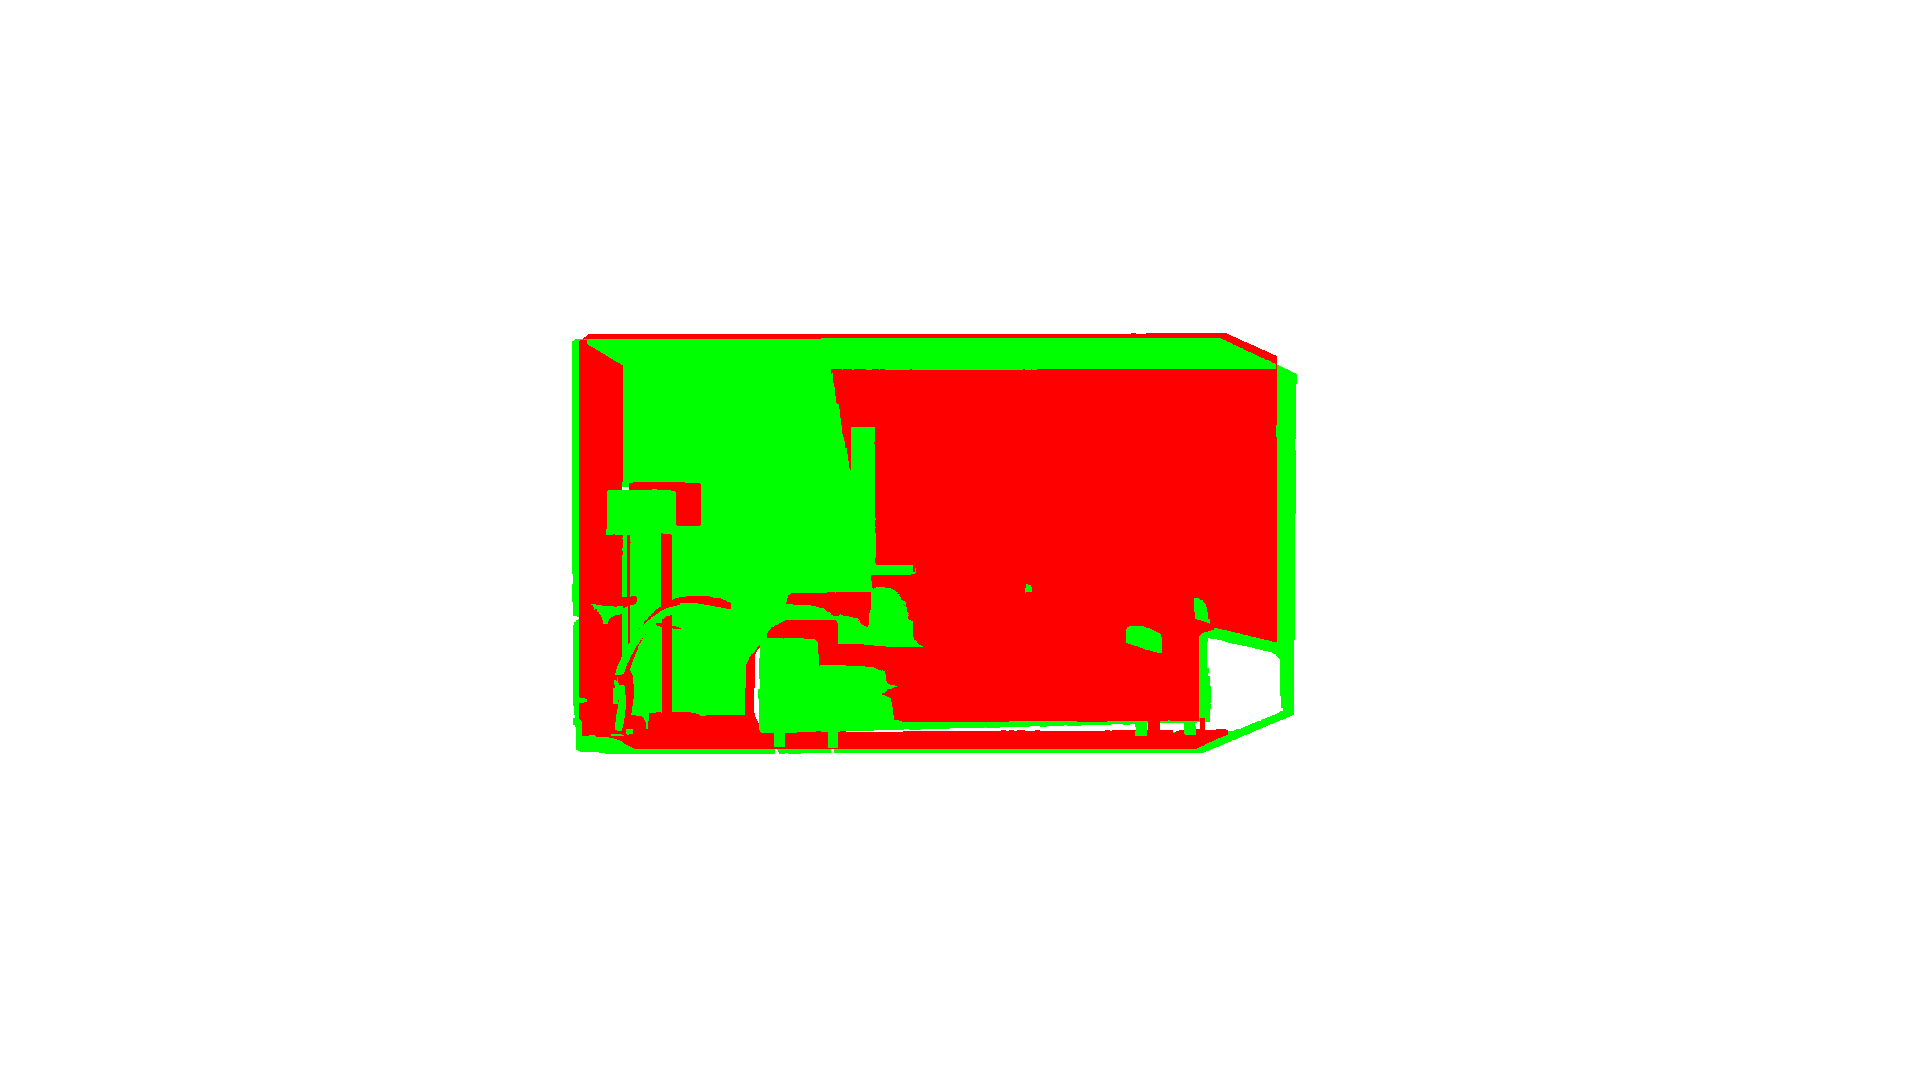
\includegraphics[width=0.8\textwidth]{Before_1_50.png}
    \caption{Frames 10 and 50 Before Optimization}
\end{figure}
\begin{figure}[!htb]
    \centering
    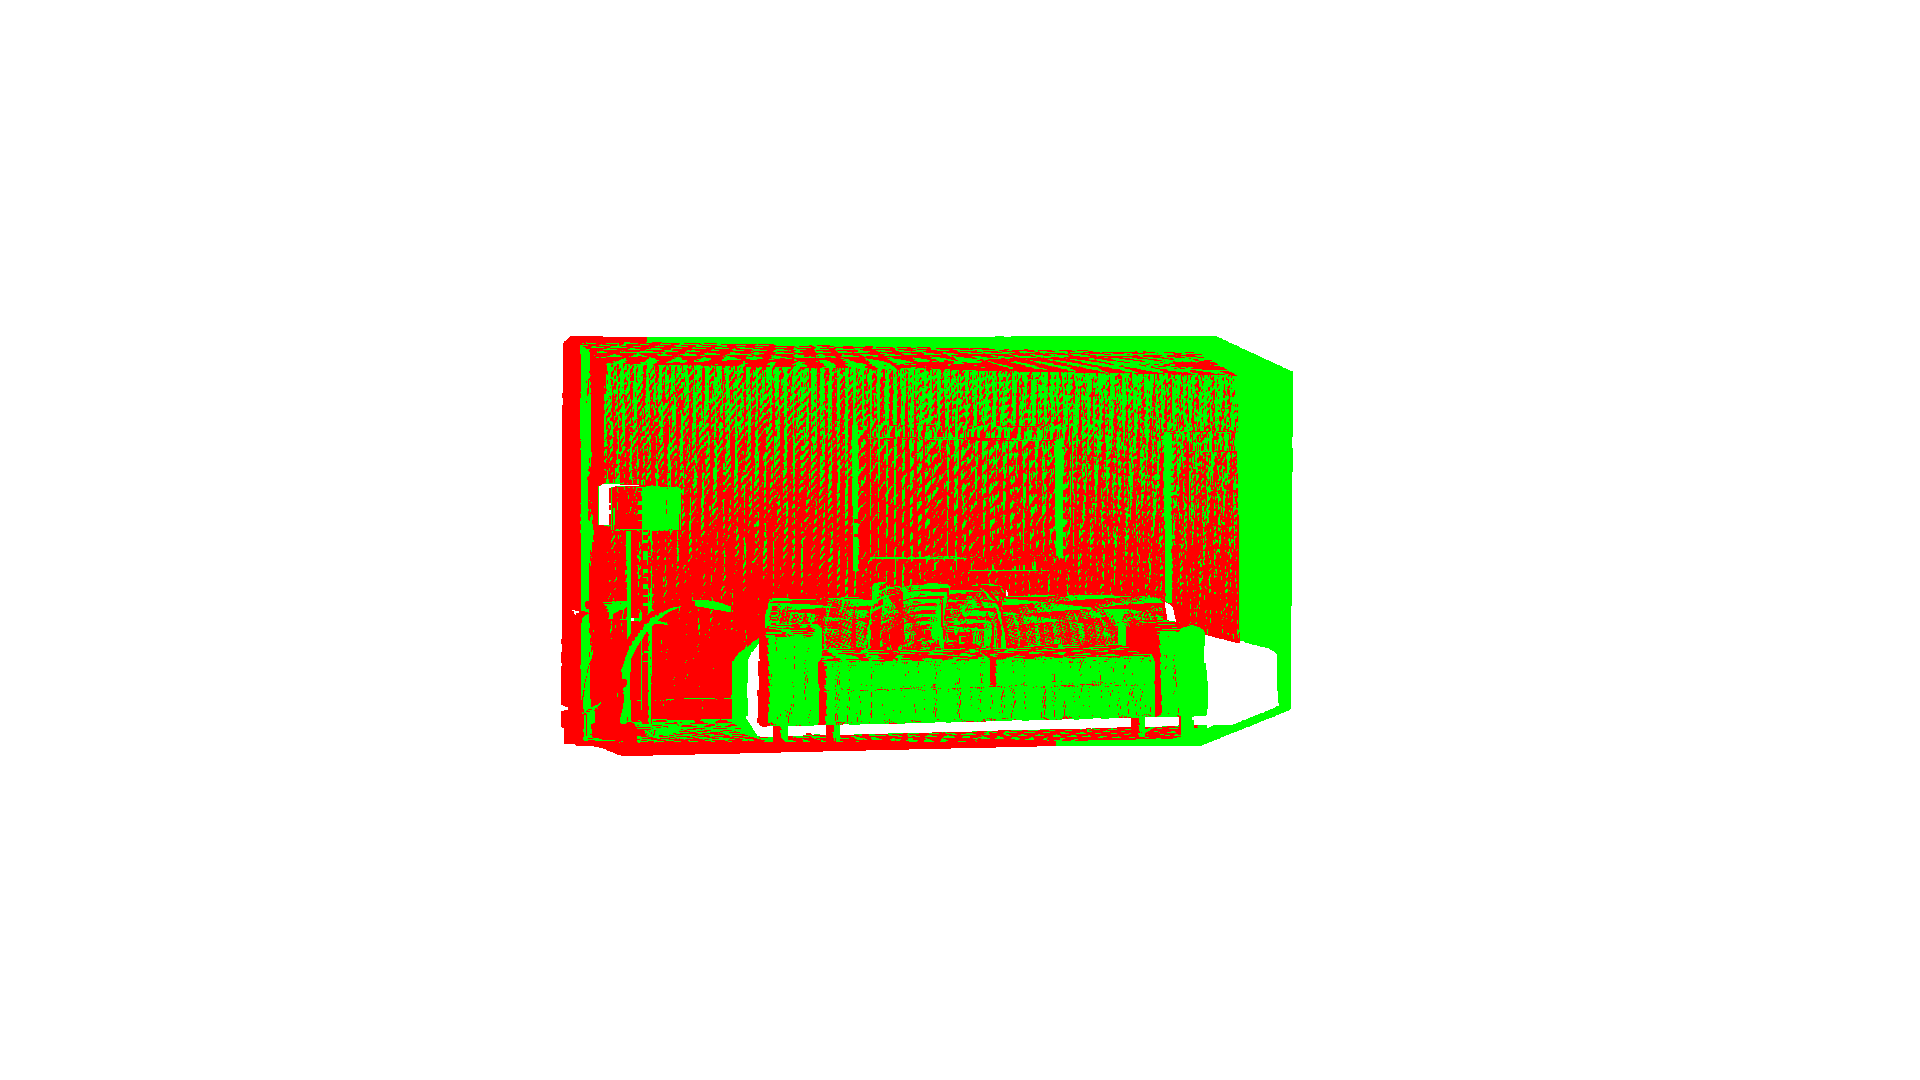
\includegraphics[width=0.8\textwidth]{After_1_50.png}
    \caption{Frames 10 and 50 After Optimization}
\end{figure}
\clearpage
\begin{figure}[!htb]
    \centering
    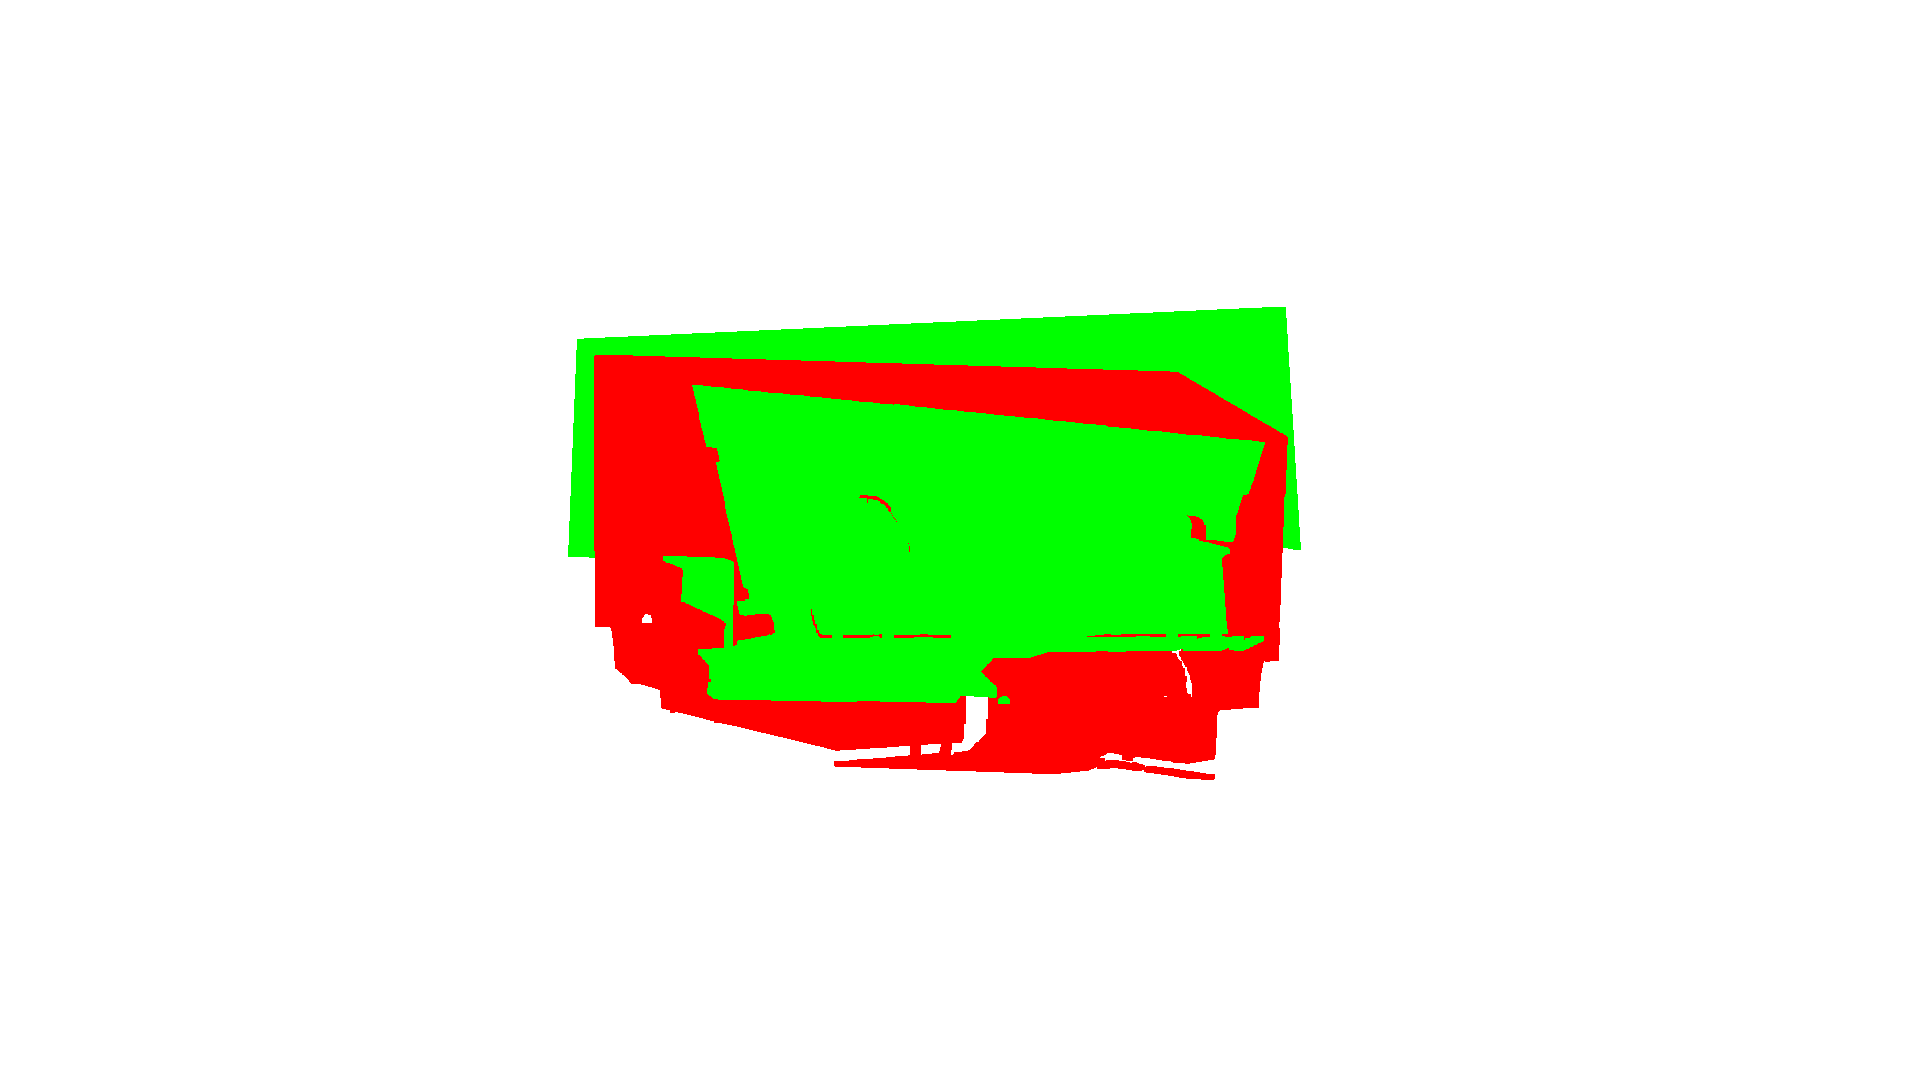
\includegraphics[width=0.8\textwidth]{150_300_Before.png}
    \caption{Frames 150 and 300 Before Optimization}
\end{figure}
\begin{figure}[!htb]
    \centering
    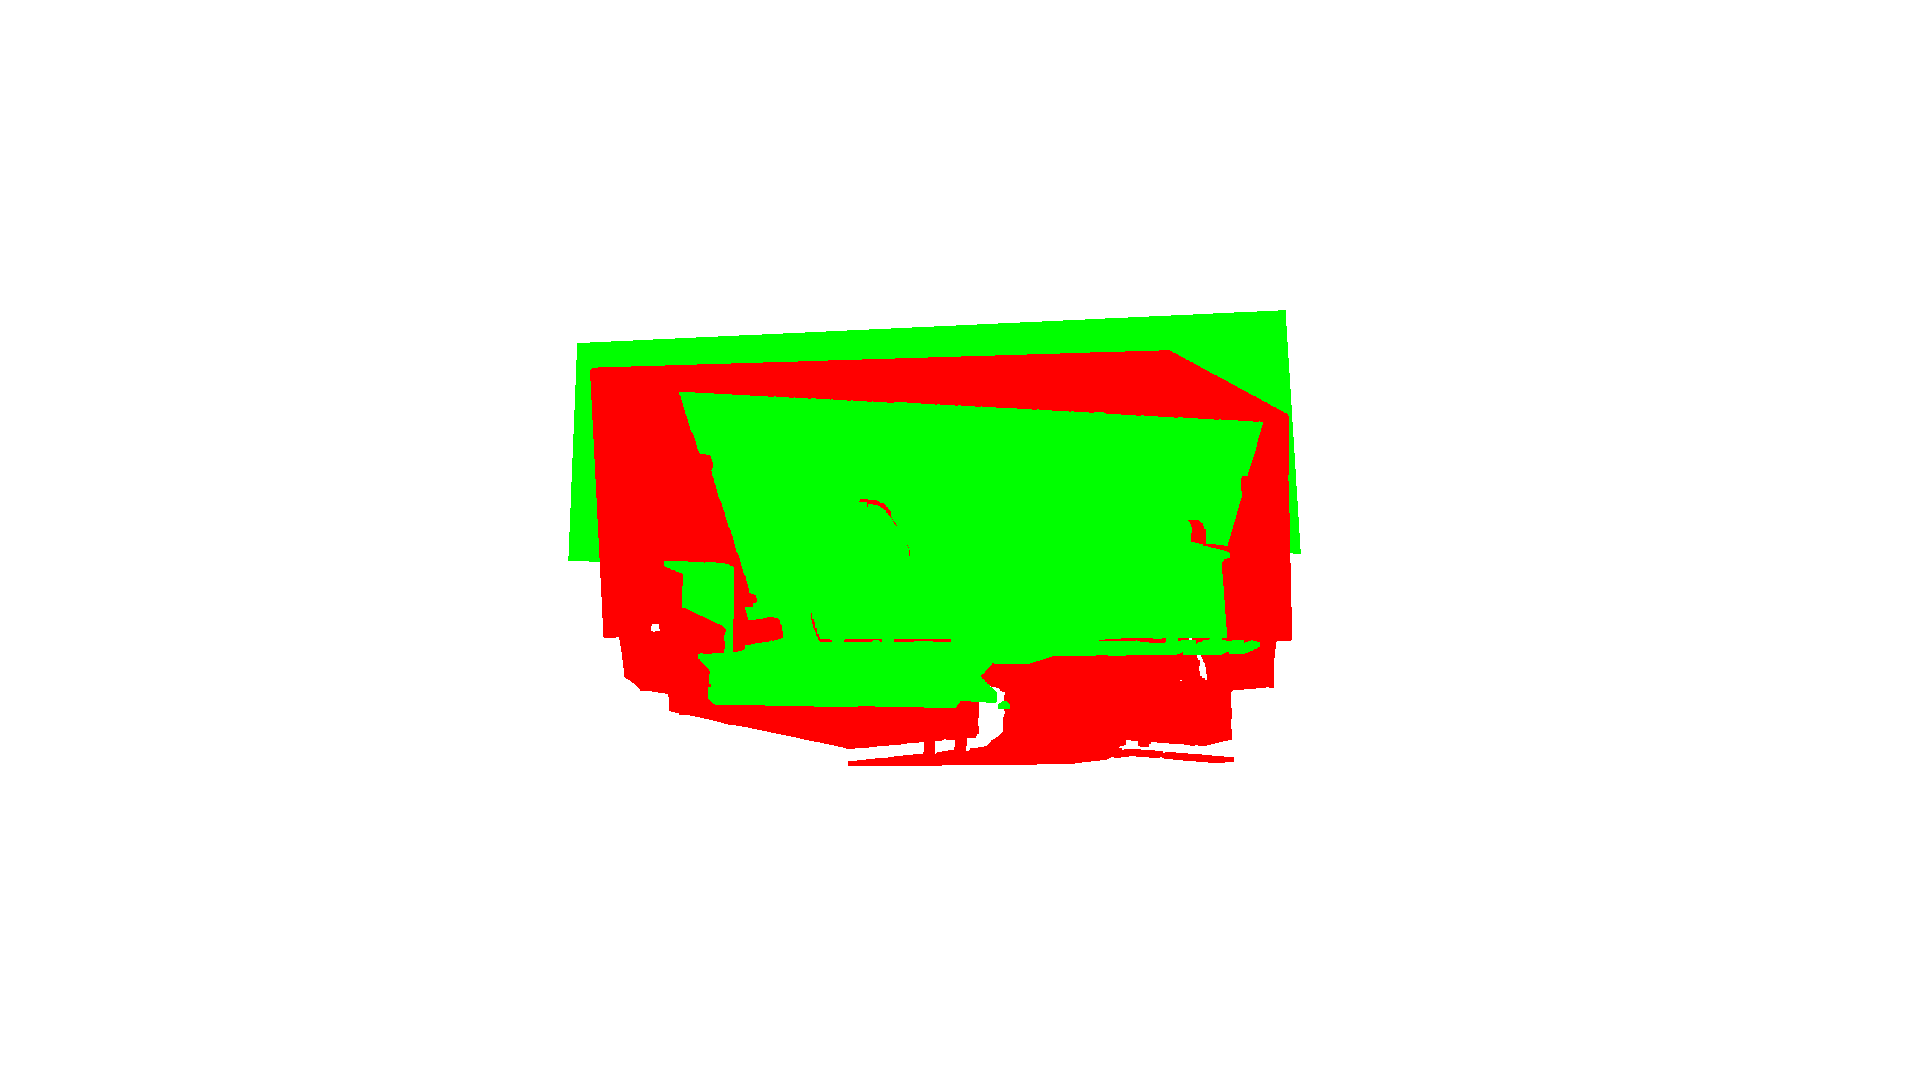
\includegraphics[width=0.8\textwidth]{150_300_After.png}
    \caption{Frames 150 and 300 After Optimization}
\end{figure}
\paragraph{Analysis}
The frames 10 and 50 are able to be aligned very well because of the small angle assumption. That is, there is not much rotation between the two frames. However, in frames 150 and 300, we can see that there is a rather large rotation between the two frames and some parallax effects. For example, see the bottom left and top left corner of the wall, there is a large rotation between those two points. Whereas, for frames 10 and 50, they are extremely close and the rotation is much smaller so the assumption is more valid in this case.

\section{Point Based Fusion}
\subsection{Merge}
\subsubsection{Weighted Average of Positions}
$$q_{world} = R_c^w q + t_c^w$$
$$p = \frac{q_{world} + w * p}{w + 1}$$

\subsubsection{Weighted Average of Colors}
$$p_c = \frac{q_c + w * p_c}{w + 1}$$

\subsubsection{Weight Average of Normals}
$$n_{q_{world}} = R_c^w n_{q}$$
$$n_p = norm(\frac{w * n_p + n_{q_{world}}}{w + 1})$$

\subsubsection{Updating Weights}
$$w[idx] = w + 1$$

\subsubsection{Compression Ratio}
$$Ratio = \frac{N}{(frame_{T} - frame_{0}) * H * W}$$
$$N = len(p_{map})$$

\textbf{Number Points: 1362157}

\textbf{Compression Rate: 0.08912773502931323}

\subsubsection{Addition}
Those entries that are new are concatenated to the numpy arrays with $w = 1$. See the code for more additional details.

\subsection{Results}
\begin{figure}[!htb]
    \centering
    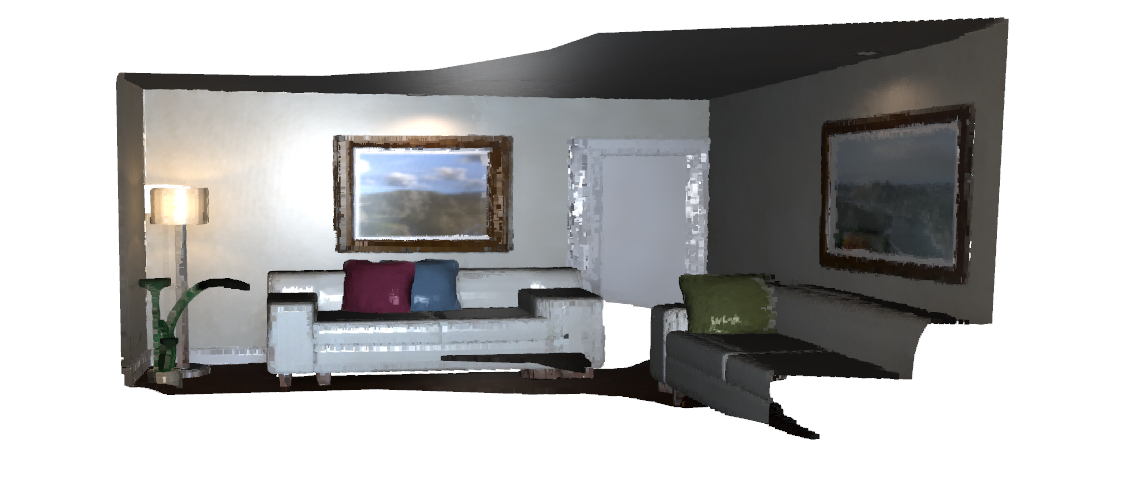
\includegraphics[width=0.8\textwidth]{FusionVis.PNG}
    \caption{Visualization of Point-Based Map with Colors}
\end{figure}
\begin{figure}[!htb]
    \centering
    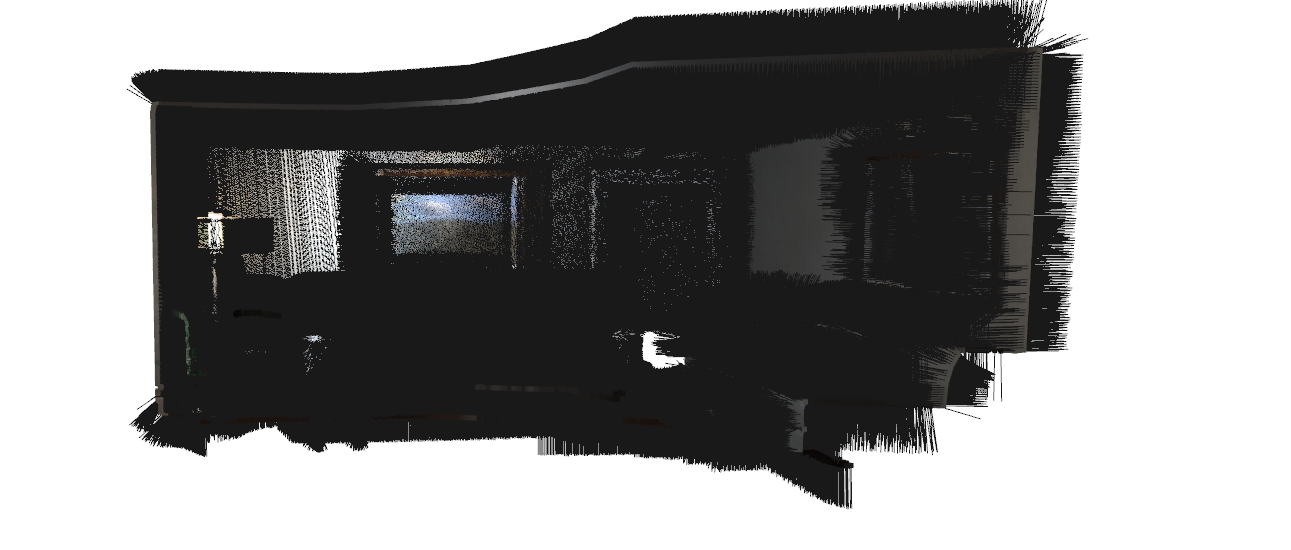
\includegraphics[width=0.8\textwidth]{NormalMap.PNG}
    \caption{Visualization of Point-Based Normal Map}
\end{figure}

\clearpage
\section{Dense SLAM}
\subsection{Source and Target}
The source here is the map and the target is the RGB-D frame. I don't really think a swap is possible because when looking for valid correspondence, we need to pass the filter which assumes we are projecting the 3D points to a 2D plane. If you swapped the role, when performing ICP, nothing would be theoretically filtered out in filter one and, in general, would require a completely different strategy if this behavior was desired.

\subsubsection{Visualization}

\subsubsection{Reducing Drift}
I chose to do the following:
\begin{enumerate}
    \item If points were not updated in the past 20 timesteps, remove them to mitigate drift
\end{enumerate}
\end{document}